\section{Regression}
\subsection{What is a model?}
In ML, we use the term \textbf{model} for any mathematical function that explains the data:\\ 
$y_i = f(x_i)$\\ 
$y_i = f(x_i) + \epsilon_i$\\ 
where $\epsilon_i$ is unexplained noise. It is often assumed that $\epsilon_i$ follows a normal distribution.\\ 
Instead of approximating $y_i$, we calculate an \textbf{estimate} $\hat{y_i}$ (y hat) of the usually unknown $y_i$: \\
\begin{center}
    $\hat{y_i} = f(x)$
\end{center}

\subsubsection{Linear Regression}
\begin{itemize}
    \item Only consideres a linear relationship between input and output
    \item In the simplest case, $x$ and $y$ are scalars and the linear model therefore has only two free parameters
    \item The goal is to identify $a$ (slope) and $b$ (intercept) for which the linear model best explains the data
\end{itemize}
\begin{center}
    $\hat{y_i} = ax_i + b$\\
\end{center}

\subsubsection{Mean Squared Error (MSE)}
\begin{itemize}
    \item Loss we want to minimize
    \item Usually divided by 2
\end{itemize}
\begin{center}
    $\hat{y_i} = ax_i + b$\\ 
    $e_i = y_i - \hat{y_i}$ \\ 
    The difference $e_i$, called residual\\ 
    $E = \frac{1}{2N} * \displaystyle\sum_{i = 1}^{N} e_i^2$\\
    $E = \frac{1}{2N} * \large\displaystyle\sum_{i = 1}^{N}(\hat{y_i} - (a*x_i + b))^2$
\end{center}

\subsubsection{Correlation and Causality}
\begin{itemize}
    \item Correlation is not causality
    \item Correlation refers to the degree to which a pair of variables are linearly related
    \item Linear regression is a tool to detect correlations between two or more variables
    \item Correlation can be quantified using the Pearson correlation coefficient
\end{itemize}
\textbf{Pearson Correlation Coefficient:}\\
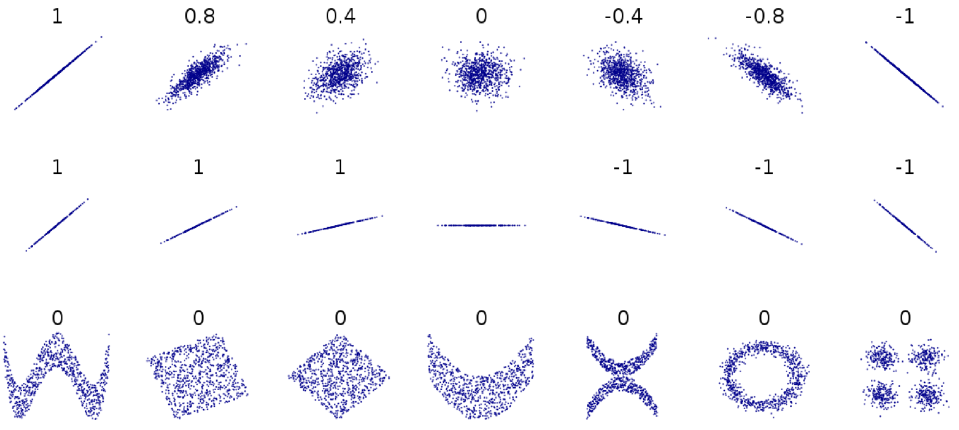
\includegraphics[width=0.6\linewidth]{./img/pearson.png}